% =====================================================================
\chapter{Estudo de caso: Insertion Sort}\label{cap:09}
\naaula{29 a 36}

Este capítulo junta tudo o que vimos: contagem de operações, somatórios, as notações e os casos.
O personagem é um algoritmo de ordenação simples e muito usado na prática, o \textbf{Insertion
Sort} (ordenação por inserção), cujo custo depende fortemente de como os dados chegam.

\section{A ideia: arrumar cartas na mão}

Pense em como você arruma cartas de baralho recebidas uma a uma: a parte da mão que você já
arrumou fica em ordem; quando chega uma carta nova, você a compara com as da direita para a
esquerda, abre espaço e a encaixa no lugar certo. O Insertion Sort faz exatamente isso num vetor:

\begin{enumerate}
  \item A parte da esquerda do vetor (no começo, só o primeiro elemento) já está ordenada.
  \item Pegamos o próximo elemento — a \textbf{chave}.
  \item Deslocamos para a direita todos os elementos ordenados maiores que a chave.
  \item Colocamos a chave no espaço que sobrou.
\end{enumerate}

\begin{conexao}
Os passos 3 e 4 são o \codigo{inserir(pos, valor)} da lista contígua da Aula 1: para inserir no
meio, é preciso deslocar os elementos seguintes. O Insertion Sort é uma sequência de
\enquote{inserções no lugar certo}, e o custo dele vem justamente desses deslocamentos.
\end{conexao}

\section{O código}

\begin{lstlisting}
def insertion_sort(v):
    for i in range(1, len(v)):
        chave = v[i]
        j = i - 1
        while j >= 0 and v[j] > chave:
            v[j + 1] = v[j]      # desloca para a direita
            j -= 1
        v[j + 1] = chave         # encaixa a chave
\end{lstlisting}

\begin{lstlisting}[style=c]
void insertion_sort(int v[], int n) {
    for (int i = 1; i < n; i++) {
        int chave = v[i];
        int j = i - 1;
        while (j >= 0 && v[j] > chave) {
            v[j + 1] = v[j];     /* desloca para a direita */
            j--;
        }
        v[j + 1] = chave;        /* encaixa a chave */
    }
}
\end{lstlisting}

Para analisar, vamos contar duas coisas: as \textbf{comparações} (cada avaliação de
\codigo{v[j] > chave}) e os \textbf{deslocamentos} (cada \codigo{v[j + 1] = v[j]}).

\section{Passo a passo}

\begin{figure}[!htb]
\centering
\begin{tikzpicture}[scale=0.62]
  \linhaIns{0}{5,2,4,6,1,3}{1}{0}{início: a parte ordenada é só o 5}
  \linhaIns{-1.3}{2,5,4,6,1,3}{2}{1}{passada 1, chave 2: 1 comparação, 1 deslocamento}
  \linhaIns{-2.6}{2,4,5,6,1,3}{3}{2}{passada 2, chave 4: 2 comparações, 1 deslocamento}
  \linhaIns{-3.9}{2,4,5,6,1,3}{4}{4}{passada 3, chave 6: 1 comparação, 0 deslocamentos}
  \linhaIns{-5.2}{1,2,4,5,6,3}{5}{1}{passada 4, chave 1: 4 comparações, 4 deslocamentos}
  \linhaIns{-6.5}{1,2,3,4,5,6}{6}{3}{passada 5, chave 3: 4 comparações, 3 deslocamentos}
\end{tikzpicture}
\caption{Ordenando $[5, 2, 4, 6, 1, 3]$. Em verde, a parte ordenada; em laranja, onde a chave foi
encaixada. Total: 12 comparações e 9 deslocamentos.}
\end{figure}

Repare na passada 4: a chave 1 é menor que todos os ordenados, então é comparada com os quatro,
todos se deslocam, e o laço para porque \codigo{j} chega a $-1$ (sem uma quinta comparação). Na
passada 3, a chave 6 já é maior que o último ordenado: uma comparação, nenhum deslocamento.

\section{Melhor caso: o vetor já está ordenado}

\begin{figure}[!htb]
\centering
\begin{minipage}{0.48\textwidth}\centering
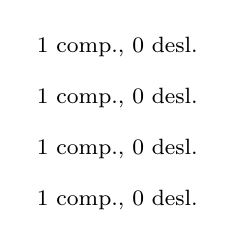
\begin{tikzpicture}[scale=0.5]
  \linhaIns{0}{1,2,3,4,5}{1}{0}{}
  \linhaIns{-1.3}{1,2,3,4,5}{2}{2}{}
  \linhaIns{-2.6}{1,2,3,4,5}{3}{3}{}
  \linhaIns{-3.9}{1,2,3,4,5}{4}{4}{}
  \linhaIns{-5.2}{1,2,3,4,5}{5}{5}{}
  \foreach \k in {1,...,4} \node[anchor=west, font=\footnotesize] at (5.2, -\k*1.3+0.45) {1 comp., 0 desl.};
\end{tikzpicture}
\par\small\textbf{Melhor caso:} $[1, 2, 3, 4, 5]$
\end{minipage}\hfill
\begin{minipage}{0.48\textwidth}\centering
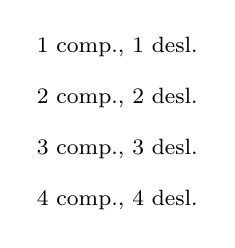
\begin{tikzpicture}[scale=0.5]
  \linhaIns{0}{5,4,3,2,1}{1}{0}{}
  \linhaIns{-1.3}{4,5,3,2,1}{2}{1}{}
  \linhaIns{-2.6}{3,4,5,2,1}{3}{1}{}
  \linhaIns{-3.9}{2,3,4,5,1}{4}{1}{}
  \linhaIns{-5.2}{1,2,3,4,5}{5}{1}{}
  \foreach \k in {1,...,4} \node[anchor=west, font=\footnotesize] at (5.2, -\k*1.3+0.45) {\k\ comp., \k\ desl.};
\end{tikzpicture}
\par\small\textbf{Pior caso:} $[5, 4, 3, 2, 1]$
\end{minipage}
\caption{À esquerda, cada chave já está no lugar: uma comparação por passada. À direita, cada
chave precisa ir até o início: as passadas custam 1, 2, 3 e 4.}
\end{figure}

Se o vetor já está em ordem crescente, cada chave é comparada só com o elemento à sua esquerda,
descobre que já está no lugar e nenhum deslocamento acontece. São $n - 1$ passadas com 1
comparação cada:
\[
T_{\text{melhor}}(n) = n - 1 \text{ comparações} \qquad\Longrightarrow\qquad T_{\text{melhor}}(n) = \Theta(n).
\]

\section{Pior caso: ordem inversa}

Se o vetor está em ordem decrescente, cada chave é menor que todos os já ordenados: na passada
$i$, ela é comparada com os $i$ elementos da esquerda e todos se deslocam. Somando as passadas —
a soma de Gauss do capítulo 3:
\[
T_{\text{pior}}(n) = 1 + 2 + \dots + (n-1) = \frac{n(n-1)}{2} \text{ comparações}
\qquad\Longrightarrow\qquad T_{\text{pior}}(n) = \Theta(n^2).
\]
Para $n = 1.000$, são 499.500 comparações — contra 999 do melhor caso.

\section{Caso médio: ordem aleatória}

Com os dados embaralhados, cada chave, em média, é maior que metade dos elementos já ordenados e
menor que a outra metade. Então ela anda, em média, metade do caminho: na passada $i$, cerca de
$i/2$ comparações. Somando, chegamos à metade do pior caso:
\[
T_{\text{médio}}(n) \approx \frac{1}{2} \cdot \frac{n(n-1)}{2} \approx \frac{n^2}{4}
\qquad\Longrightarrow\qquad T_{\text{médio}}(n) = \Theta(n^2).
\]

\begin{center}
\begin{tabularx}{0.95\textwidth}{C C C C C}
\cab \tcx{$n$} & \tc{Ordenado} & \tc{Aleatório (medido)} & \tc{Invertido} & \tcx{$n^2/4$} \\
10 & 9 & 30 & 45 & 25 \\
\rowcolor{edfundo} 100 & 99 & 2.607 & 4.950 & 2.500 \\
1.000 & 999 & 252.249 & 499.500 & 250.000 \\

\end{tabularx}
\end{center}

\begin{figure}[!htb]
  \centering
  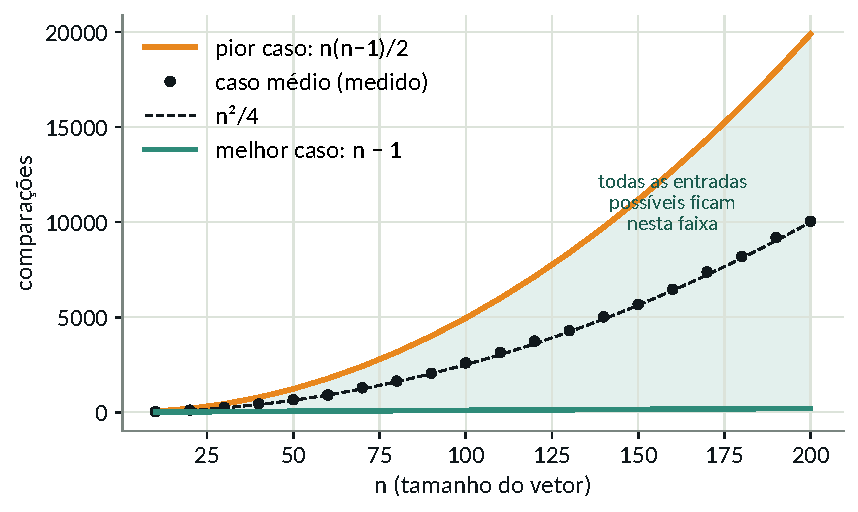
\includegraphics[width=0.74\textwidth]{figuras/f09_insertion_casos.pdf}
  \caption{Comparações do Insertion Sort nos três cenários. O caso médio (pontos) acompanha
  $n^2/4$, e o melhor caso quase não sai do chão.}
\end{figure}

\begin{atencao}
Metade do pior caso continua sendo quadrático! Dividir por 2 é multiplicar por uma constante, e
constantes não mudam a família. Em média, o Insertion Sort é tão \enquote{quadrático} quanto no pior
caso — só com a metade do trabalho.
\end{atencao}

\section{Vendo na prática}

O programa \codigo{python/insertion_sort.py} (e a versão em C) faz o passo a passo e conta as
comparações nos três cenários. Esta é a saída real:

\needspace{22\baselineskip}
\lstinputlisting[style=terminal]{tabelas/saida_insertion.txt}

Os números do caso aleatório mudam um pouco entre o Python e o C, porque os dois usam geradores
de números aleatórios diferentes. Mas ambos ficam perto de $n^2/4$.

\section{Onde entram \texorpdfstring{$O$, $\Omega$ e $\Theta$}{O, Ω e Θ}}

Este é o ponto que mais confunde — e o Insertion Sort é o exemplo perfeito para esclarecê-lo.

\begin{itemize}
  \item Cada \textbf{caso} é uma função diferente: $T_{\text{melhor}}(n) = n - 1$ e
        $T_{\text{pior}}(n) = \dfrac{n(n-1)}{2}$.
  \item Cada função pode ser descrita com a notação $\Theta$:
        $T_{\text{melhor}}(n) = \Theta(n)$ e $T_{\text{pior}}(n) = \Theta(n^2)$.
  \item Para \textbf{qualquer} entrada, o custo fica na faixa entre essas duas curvas (a região
        destacada na figura acima). Então podemos dizer: o custo do Insertion Sort é
        $O(n^2)$ (nunca passa do pior caso) e $\Omega(n)$ (nunca fica abaixo do melhor caso).
\end{itemize}

\begin{atencao}
Não diga \enquote{o Insertion Sort é $\Theta(n^2)$} sem dizer de qual caso está falando: no melhor
caso ele é $\Theta(n)$! Frases corretas: \enquote{o pior caso do Insertion Sort é $\Theta(n^2)$};
\enquote{o Insertion Sort é $O(n^2)$}; \enquote{o melhor caso é $\Theta(n)$}. E lembre: $O$ não é
sinônimo de pior caso, nem $\Omega$ de melhor caso — são as notações que usamos para descrever
cada caso.
\end{atencao}

\section{Dados quase ordenados}

O melhor caso não é só uma curiosidade. Muitos dados reais chegam \emph{quase} ordenados: uma
lista de chamada com um aluno novo no fim, um histórico em que só o último registro está fora do
lugar. Nesses casos, o Insertion Sort faz pouco mais que $n$ comparações.

\begin{aprofunde}
Chamamos de \textbf{inversão} cada par de elementos fora de ordem (um maior antes de um menor).
Cada deslocamento do Insertion Sort desfaz exatamente uma inversão; por isso o número de
deslocamentos é igual ao número de inversões do vetor. Um vetor ordenado tem 0 inversões; um
invertido tem o máximo, $\dfrac{n(n-1)}{2}$; um embaralhado tem, em média, $\dfrac{n(n-1)}{4}$.
Por isso o \codigo{sort()} do Python (um algoritmo chamado Timsort) usa o Insertion Sort em
trechos pequenos: nesses trechos, ele é o mais rápido.
\end{aprofunde}

\begin{exrapido}
Aplique o Insertion Sort a $[1, 2, 3, 5, 4]$. Quantas comparações e quantos deslocamentos são
feitos? O resultado está mais perto do melhor ou do pior caso?
\end{exrapido}

\begin{exrapido}
(a) Para $n = 8$, quantas comparações o Insertion Sort faz no melhor caso? E no pior?
(b) Quantos deslocamentos são feitos para ordenar $[4, 3, 2, 1]$?
\end{exrapido}

\begin{respostas}
  \resp{9.1} Passadas 1, 2 e 3 (chaves 2, 3 e 5): 1 comparação cada, nenhum deslocamento.
  Passada 4 (chave 4): compara com 5 (desloca) e com 3 (para): 2 comparações e 1 deslocamento.
  Total: 5 comparações e 1 deslocamento — quase o melhor caso ($n - 1 = 4$). O vetor tinha uma
  única inversão (o par 5, 4).
  \resp{9.2} (a) Melhor caso: $8 - 1 = 7$; pior caso: $\dfrac{8 \cdot 7}{2} = 28$.
  (b) $1 + 2 + 3 = 6$ deslocamentos (é o pior caso para $n = 4$).
\end{respostas}
